%! TEX encoding = utf8
\chapter{Algorytm DMC}

Prawo regulacji DMC przedstawia się następująco:

\begin{equation}
\triangle U(k)=K(Y^{zad}(k)-Y^0(k))
\end{equation}

Gdzie $\triangle U(k)$ to wektor $N_u$ (horyzont sterowania) przyszłych wartości sterowania, $Y^0(k)$ to przewidywana odpowiedź z modelu procesu, $K$ - macierz policzona raz na początku ze współczynników odpowiedzi skokowej, uwzględniając wybrany współczynnik $\lambda$ oraz horyzonty predykcji i sterowania.

W przypadku algorytmu DMC z pomiarem zakłóceń $Y^0(k)$ oblicza się z następującego wzoru:
\begin{equation}
Y^0(k)=Y(k)+M^P \triangle U^P(k)+M^{Z^P}\triangle Z^P(k)
\end{equation}

W powyższym wzorze dwa pierwsze elementy sumy odnoszą się do toru sterowanie-wyjście a ostatni element do toru zakłócenie-wyjście: $M^{Z^P}$ macierz wyznaczana przy pomocy współczynników odpowiedzi skokowej dla zakłócenia, $\triangle Z^P(k)$ jest wektorem przyrostów mierzalnego zakłócenia.


\section{Strojenie regulatora}
Strojenie regulatora odwywało się przy skokowej zmianie sygnału wartości zadanej z  0 do 1 (w chwili k=30) oraz zerowym zakłóceniu.

Choryzont dynamiki określono z odpowiedzi skowej toru sterowanie-wyjście (k dla którego wyjście się ustabilizowało): D=155.
Kolejne parametry były modyfikowane do momentu uzyskania zadowalających efektów. Na początku przyjęto $N=N_u=D=155$ oraz $\lambda=1$, następnie zmniejszano kolejno wartość N i $N_U$. Na końcu modyfikowano wartości $\lambda$.

\section{Wyniki strojenia}

\begin{figure}[H]
\centering
% This file was created by matlab2tikz.
%
%The latest updates can be retrieved from
%  http://www.mathworks.com/matlabcentral/fileexchange/22022-matlab2tikz-matlab2tikz
%where you can also make suggestions and rate matlab2tikz.
%
\definecolor{mycolor1}{rgb}{0.00000,0.44700,0.74100}%
%
\begin{tikzpicture}

\begin{axis}[%
width=4.272in,
height=1.075in,
at={(0.717in,1.839in)},
scale only axis,
xmin=0,
xmax=80,
xlabel style={font=\color{white!15!black}},
xlabel={k},
ymin=0,
ymax=1.5,
ylabel style={font=\color{white!15!black}},
ylabel={U(k)},
axis background/.style={fill=white}
]
\addplot[const plot, color=mycolor1, forget plot] table[row sep=crcr] {%
1	0\\
2	0\\
3	0\\
4	0\\
5	0\\
6	0\\
7	0\\
8	0\\
9	0\\
10	0\\
11	0\\
12	0\\
13	0\\
14	0\\
15	0\\
16	0\\
17	0\\
18	0\\
19	0\\
20	0\\
21	0\\
22	0\\
23	0\\
24	0\\
25	0\\
26	0\\
27	0\\
28	0\\
29	0\\
30	0.779619916882743\\
31	1.18170477741642\\
32	1.32155598565414\\
33	1.29533783386638\\
34	1.1771848072349\\
35	1.02008731337989\\
36	0.858835876827432\\
37	0.71380296740774\\
38	0.594767794604657\\
39	0.504324706750564\\
40	0.440660529538547\\
41	0.399650849293106\\
42	0.376325172608509\\
43	0.365802277133205\\
44	0.363814769546016\\
45	0.366938267236832\\
46	0.37262525543067\\
47	0.37912335053477\\
48	0.385336888305099\\
49	0.390672061811568\\
50	0.394890507210185\\
51	0.397984600538876\\
52	0.400079546613239\\
53	0.401362076582049\\
54	0.402032581494507\\
55	0.402276165720336\\
56	0.402247856490658\\
57	0.402067613477059\\
58	0.40182151764688\\
59	0.401566356546532\\
60	0.401335623139203\\
61	0.401145631373442\\
62	0.401000993469431\\
63	0.400899100774764\\
64	0.400833518268962\\
65	0.400796366541266\\
66	0.400779850188358\\
67	0.400777121928368\\
68	0.400782667258278\\
69	0.400792370617573\\
70	0.400803391817569\\
71	0.400813948236701\\
72	0.400823068253618\\
73	0.400830356670936\\
74	0.400835794049371\\
75	0.400839578575782\\
76	0.400842010491531\\
77	0.400843414188603\\
78	0.400844090832355\\
79	0.400844293907319\\
80	0.40084422069481\\
};
\end{axis}

\begin{axis}[%
width=4.272in,
height=1.075in,
at={(0.717in,0.346in)},
scale only axis,
xmin=0,
xmax=80,
xlabel style={font=\color{white!15!black}},
xlabel={k},
ymin=-1,
ymax=1,
ylabel style={font=\color{white!15!black}},
ylabel={Z(k)},
axis background/.style={fill=white}
]
\addplot[const plot, color=mycolor1, forget plot] table[row sep=crcr] {%
1	0\\
2	0\\
3	0\\
4	0\\
5	0\\
6	0\\
7	0\\
8	0\\
9	0\\
10	0\\
11	0\\
12	0\\
13	0\\
14	0\\
15	0\\
16	0\\
17	0\\
18	0\\
19	0\\
20	0\\
21	0\\
22	0\\
23	0\\
24	0\\
25	0\\
26	0\\
27	0\\
28	0\\
29	0\\
30	0\\
31	0\\
32	0\\
33	0\\
34	0\\
35	0\\
36	0\\
37	0\\
38	0\\
39	0\\
40	0\\
41	0\\
42	0\\
43	0\\
44	0\\
45	0\\
46	0\\
47	0\\
48	0\\
49	0\\
50	0\\
51	0\\
52	0\\
53	0\\
54	0\\
55	0\\
56	0\\
57	0\\
58	0\\
59	0\\
60	0\\
61	0\\
62	0\\
63	0\\
64	0\\
65	0\\
66	0\\
67	0\\
68	0\\
69	0\\
70	0\\
71	0\\
72	0\\
73	0\\
74	0\\
75	0\\
76	0\\
77	0\\
78	0\\
79	0\\
80	0\\
};
\end{axis}
\end{tikzpicture}%
\caption{Zakłócenie i sygnał sterujący przy parametrach regulatora: $N=155$ $N_u=155$ $\lambda=1$}
\end{figure}

\begin{figure}[H]
\centering
\input{rysunki/strojenie_155_155_1_8.809637e+00.tex}
\caption{Wyjście obiektu przy parametrach regulatora: $N=155$ $N_u=155$ $\lambda=1$, błąd $E=8,809637$}
\end{figure}


\begin{figure}[H]
\centering
% This file was created by matlab2tikz.
%
%The latest updates can be retrieved from
%  http://www.mathworks.com/matlabcentral/fileexchange/22022-matlab2tikz-matlab2tikz
%where you can also make suggestions and rate matlab2tikz.
%
\definecolor{mycolor1}{rgb}{0.00000,0.44700,0.74100}%
%
\begin{tikzpicture}

\begin{axis}[%
width=4.272in,
height=1.075in,
at={(0.717in,1.839in)},
scale only axis,
xmin=0,
xmax=80,
xlabel style={font=\color{white!15!black}},
xlabel={k},
ymin=0,
ymax=1.5,
ylabel style={font=\color{white!15!black}},
ylabel={U(k)},
axis background/.style={fill=white}
]
\addplot[const plot, color=mycolor1, forget plot] table[row sep=crcr] {%
1	0\\
2	0\\
3	0\\
4	0\\
5	0\\
6	0\\
7	0\\
8	0\\
9	0\\
10	0\\
11	0\\
12	0\\
13	0\\
14	0\\
15	0\\
16	0\\
17	0\\
18	0\\
19	0\\
20	0\\
21	0\\
22	0\\
23	0\\
24	0\\
25	0\\
26	0\\
27	0\\
28	0\\
29	0\\
30	0.778977283157291\\
31	1.18121334909595\\
32	1.3214929189596\\
33	1.29568816594054\\
34	1.17780274687997\\
35	1.02079912421764\\
36	0.859495932183362\\
37	0.714316358601936\\
38	0.595091803720507\\
39	0.504459011257327\\
40	0.440633190249278\\
41	0.399504536526705\\
42	0.376105995056268\\
43	0.365552075276963\\
44	0.363566778890143\\
45	0.366715543375141\\
46	0.372441061690962\\
47	0.378982725434061\\
48	0.385238740481891\\
49	0.390611315413325\\
50	0.394859995538608\\
51	0.397976554491282\\
52	0.400086636287662\\
53	0.40137803842904\\
54	0.402052504466198\\
55	0.402296525476648\\
56	0.402266384828493\\
57	0.402083077871238\\
58	0.401833468785539\\
59	0.40157488403119\\
60	0.401341143618077\\
61	0.401148720574095\\
62	0.401002264279411\\
63	0.400899123481857\\
64	0.400832775782596\\
65	0.400795236210013\\
66	0.400778604046133\\
67	0.400775938269544\\
68	0.400781647906916\\
69	0.40079155979489\\
70	0.4008027939185\\
71	0.400813542990833\\
72	0.40082282262898\\
73	0.400830233490134\\
74	0.400835757663313\\
75	0.400839598130227\\
76	0.400842061377361\\
77	0.400843478234592\\
78	0.400844155717426\\
79	0.400844352166727\\
80	0.400844268591025\\
};
\end{axis}

\begin{axis}[%
width=4.272in,
height=1.075in,
at={(0.717in,0.346in)},
scale only axis,
xmin=0,
xmax=80,
xlabel style={font=\color{white!15!black}},
xlabel={k},
ymin=-1,
ymax=1,
ylabel style={font=\color{white!15!black}},
ylabel={Z(k)},
axis background/.style={fill=white}
]
\addplot[const plot, color=mycolor1, forget plot] table[row sep=crcr] {%
1	0\\
2	0\\
3	0\\
4	0\\
5	0\\
6	0\\
7	0\\
8	0\\
9	0\\
10	0\\
11	0\\
12	0\\
13	0\\
14	0\\
15	0\\
16	0\\
17	0\\
18	0\\
19	0\\
20	0\\
21	0\\
22	0\\
23	0\\
24	0\\
25	0\\
26	0\\
27	0\\
28	0\\
29	0\\
30	0\\
31	0\\
32	0\\
33	0\\
34	0\\
35	0\\
36	0\\
37	0\\
38	0\\
39	0\\
40	0\\
41	0\\
42	0\\
43	0\\
44	0\\
45	0\\
46	0\\
47	0\\
48	0\\
49	0\\
50	0\\
51	0\\
52	0\\
53	0\\
54	0\\
55	0\\
56	0\\
57	0\\
58	0\\
59	0\\
60	0\\
61	0\\
62	0\\
63	0\\
64	0\\
65	0\\
66	0\\
67	0\\
68	0\\
69	0\\
70	0\\
71	0\\
72	0\\
73	0\\
74	0\\
75	0\\
76	0\\
77	0\\
78	0\\
79	0\\
80	0\\
};
\end{axis}
\end{tikzpicture}%
\caption{Zakłócenie i sygnał sterujący przy parametrach regulatora: $N=20$ $N_u=20$ $\lambda=1$}
\end{figure}

\begin{figure}[H]
\centering
% This file was created by matlab2tikz.
%
%The latest updates can be retrieved from
%  http://www.mathworks.com/matlabcentral/fileexchange/22022-matlab2tikz-matlab2tikz
%where you can also make suggestions and rate matlab2tikz.
%
\definecolor{mycolor1}{rgb}{0.00000,0.44700,0.74100}%
\definecolor{mycolor2}{rgb}{0.85000,0.32500,0.09800}%
%
\begin{tikzpicture}

\begin{axis}[%
width=4.272in,
height=3.472in,
at={(0.717in,0.441in)},
scale only axis,
xmin=0,
xmax=80,
xlabel style={font=\color{white!15!black}},
xlabel={k},
ymin=0,
ymax=1.2,
ylabel style={font=\color{white!15!black}},
ylabel={Y(k)},
axis background/.style={fill=white},
legend style={legend cell align=left, align=left, draw=white!15!black}
]
\addplot[const plot, color=mycolor1] table[row sep=crcr] {%
1	0\\
2	0\\
3	0\\
4	0\\
5	0\\
6	0\\
7	0\\
8	0\\
9	0\\
10	0\\
11	0\\
12	0\\
13	0\\
14	0\\
15	0\\
16	0\\
17	0\\
18	0\\
19	0\\
20	0\\
21	0\\
22	0\\
23	0\\
24	0\\
25	0\\
26	0\\
27	0\\
28	0\\
29	0\\
30	0\\
31	0\\
32	0\\
33	0\\
34	0\\
35	0\\
36	0\\
37	0.1151951606333\\
38	0.283051773292641\\
39	0.461712586976898\\
40	0.625976203552359\\
41	0.763077218445666\\
42	0.868838429484069\\
43	0.944479246880569\\
44	0.99416733479294\\
45	1.02327767865871\\
46	1.03725709248379\\
47	1.04096605080226\\
48	1.03836953331366\\
49	1.03246323863311\\
50	1.02534301026529\\
51	1.01834823180196\\
52	1.01223103950281\\
53	1.00732081873539\\
54	1.00366705184259\\
55	1.00115332007086\\
56	0.999581663115499\\
57	0.998730255123451\\
58	0.998389164465429\\
59	0.998379450484679\\
60	0.998560523381215\\
61	0.998829938732673\\
62	0.999118885688526\\
63	0.999385730202182\\
64	0.999609188867835\\
65	0.999782077682641\\
66	0.999906109982297\\
67	0.999987894122988\\
68	1.00003607888346\\
69	1.00005948459754\\
70	1.0000660137509\\
71	1.0000621331956\\
72	1.00005274317428\\
73	1.00004128282119\\
74	1.00002995885659\\
75	1.00002001844583\\
76	1.00001201590385\\
77	1.00000604515409\\
78	1.00000192580901\\
79	0.999999341270504\\
80	0.999997933460832\\
};
\addlegendentry{Y}

\addplot[const plot, color=mycolor2] table[row sep=crcr] {%
1	0\\
2	0\\
3	0\\
4	0\\
5	0\\
6	0\\
7	0\\
8	0\\
9	0\\
10	0\\
11	0\\
12	0\\
13	0\\
14	0\\
15	0\\
16	0\\
17	0\\
18	0\\
19	0\\
20	0\\
21	0\\
22	0\\
23	0\\
24	0\\
25	0\\
26	0\\
27	0\\
28	0\\
29	0\\
30	1\\
31	1\\
32	1\\
33	1\\
34	1\\
35	1\\
36	1\\
37	1\\
38	1\\
39	1\\
40	1\\
41	1\\
42	1\\
43	1\\
44	1\\
45	1\\
46	1\\
47	1\\
48	1\\
49	1\\
50	1\\
51	1\\
52	1\\
53	1\\
54	1\\
55	1\\
56	1\\
57	1\\
58	1\\
59	1\\
60	1\\
61	1\\
62	1\\
63	1\\
64	1\\
65	1\\
66	1\\
67	1\\
68	1\\
69	1\\
70	1\\
71	1\\
72	1\\
73	1\\
74	1\\
75	1\\
76	1\\
77	1\\
78	1\\
79	1\\
80	1\\
81	1\\
82	1\\
83	1\\
84	1\\
85	1\\
86	1\\
87	1\\
88	1\\
89	1\\
90	1\\
91	1\\
92	1\\
93	1\\
94	1\\
95	1\\
96	1\\
97	1\\
98	1\\
99	1\\
100	1\\
101	1\\
102	1\\
103	1\\
104	1\\
105	1\\
106	1\\
107	1\\
108	1\\
109	1\\
110	1\\
111	1\\
112	1\\
113	1\\
114	1\\
115	1\\
116	1\\
117	1\\
118	1\\
119	1\\
120	1\\
121	1\\
122	1\\
123	1\\
124	1\\
125	1\\
126	1\\
127	1\\
128	1\\
129	1\\
130	1\\
131	1\\
132	1\\
133	1\\
134	1\\
135	1\\
136	1\\
137	1\\
138	1\\
139	1\\
140	1\\
141	1\\
142	1\\
143	1\\
144	1\\
145	1\\
146	1\\
147	1\\
148	1\\
149	1\\
150	1\\
151	1\\
152	1\\
153	1\\
154	1\\
155	1\\
156	1\\
157	1\\
158	1\\
159	1\\
160	1\\
161	1\\
162	1\\
163	1\\
164	1\\
165	1\\
166	1\\
167	1\\
168	1\\
169	1\\
170	1\\
171	1\\
172	1\\
173	1\\
174	1\\
175	1\\
176	1\\
177	1\\
178	1\\
179	1\\
180	1\\
181	1\\
182	1\\
183	1\\
184	1\\
185	1\\
186	1\\
187	1\\
188	1\\
189	1\\
190	1\\
191	1\\
192	1\\
193	1\\
194	1\\
195	1\\
196	1\\
197	1\\
198	1\\
199	1\\
200	1\\
};
\addlegendentry{Yzad}

\end{axis}
\end{tikzpicture}%
\caption{Wyjście obiektu przy parametrach regulatora: $N=20$ $N_u=20$ $\lambda=1$, błąd $E=8,810337$}
\end{figure}

\begin{figure}[H]
\centering
% This file was created by matlab2tikz.
%
%The latest updates can be retrieved from
%  http://www.mathworks.com/matlabcentral/fileexchange/22022-matlab2tikz-matlab2tikz
%where you can also make suggestions and rate matlab2tikz.
%
\definecolor{mycolor1}{rgb}{0.00000,0.44700,0.74100}%
%
\begin{tikzpicture}

\begin{axis}[%
width=4.272in,
height=1.075in,
at={(0.717in,1.839in)},
scale only axis,
xmin=0,
xmax=80,
xlabel style={font=\color{white!15!black}},
xlabel={k},
ymin=0,
ymax=1.5,
ylabel style={font=\color{white!15!black}},
ylabel={U(k)},
axis background/.style={fill=white}
]
\addplot[const plot, color=mycolor1, forget plot] table[row sep=crcr] {%
1	0\\
2	0\\
3	0\\
4	0\\
5	0\\
6	0\\
7	0\\
8	0\\
9	0\\
10	0\\
11	0\\
12	0\\
13	0\\
14	0\\
15	0\\
16	0\\
17	0\\
18	0\\
19	0\\
20	0\\
21	0\\
22	0\\
23	0\\
24	0\\
25	0\\
26	0\\
27	0\\
28	0\\
29	0\\
30	0.963061244191964\\
31	1.39398454701489\\
32	1.48115067416548\\
33	1.37348862565279\\
34	1.17777904345788\\
35	0.963226719971514\\
36	0.769239225191289\\
37	0.613798925299465\\
38	0.500957404810103\\
39	0.426796701795526\\
40	0.383727843853206\\
41	0.363294787843156\\
42	0.357785854553432\\
43	0.36098282246832\\
44	0.368345714406001\\
45	0.376871809466276\\
46	0.384801861975866\\
47	0.391287085038753\\
48	0.396082747581525\\
49	0.399299537414655\\
50	0.401220993626653\\
51	0.402182003799279\\
52	0.402497012445456\\
53	0.40242483504775\\
54	0.402157909076208\\
55	0.401826043856082\\
56	0.401507330345175\\
57	0.401241296501409\\
58	0.401041380549775\\
59	0.400905265692432\\
60	0.40082260798346\\
61	0.400780280175989\\
62	0.400765550522858\\
63	0.400767713001134\\
64	0.400778663600397\\
65	0.400792835275563\\
66	0.400806801861087\\
67	0.400818762757439\\
68	0.400828037769012\\
69	0.400834639301347\\
70	0.400838946561202\\
71	0.400841480305966\\
72	0.40084276304749\\
73	0.400843244526751\\
74	0.40084327245048\\
75	0.400843091423736\\
76	0.400842857005025\\
77	0.400842655791527\\
78	0.400842525849758\\
79	0.400842474425089\\
80	0.400842491689809\\
};
\end{axis}

\begin{axis}[%
width=4.272in,
height=1.075in,
at={(0.717in,0.346in)},
scale only axis,
xmin=0,
xmax=80,
xlabel style={font=\color{white!15!black}},
xlabel={k},
ymin=-1,
ymax=1,
ylabel style={font=\color{white!15!black}},
ylabel={Z(k)},
axis background/.style={fill=white}
]
\addplot[const plot, color=mycolor1, forget plot] table[row sep=crcr] {%
1	0\\
2	0\\
3	0\\
4	0\\
5	0\\
6	0\\
7	0\\
8	0\\
9	0\\
10	0\\
11	0\\
12	0\\
13	0\\
14	0\\
15	0\\
16	0\\
17	0\\
18	0\\
19	0\\
20	0\\
21	0\\
22	0\\
23	0\\
24	0\\
25	0\\
26	0\\
27	0\\
28	0\\
29	0\\
30	0\\
31	0\\
32	0\\
33	0\\
34	0\\
35	0\\
36	0\\
37	0\\
38	0\\
39	0\\
40	0\\
41	0\\
42	0\\
43	0\\
44	0\\
45	0\\
46	0\\
47	0\\
48	0\\
49	0\\
50	0\\
51	0\\
52	0\\
53	0\\
54	0\\
55	0\\
56	0\\
57	0\\
58	0\\
59	0\\
60	0\\
61	0\\
62	0\\
63	0\\
64	0\\
65	0\\
66	0\\
67	0\\
68	0\\
69	0\\
70	0\\
71	0\\
72	0\\
73	0\\
74	0\\
75	0\\
76	0\\
77	0\\
78	0\\
79	0\\
80	0\\
};
\end{axis}
\end{tikzpicture}%
\caption{Zakłócenie i sygnał sterujący przy parametrach regulatora: $N=50$ $N_u=5$ $\lambda=1$}
\end{figure}

\begin{figure}[H]
\centering
% This file was created by matlab2tikz.
%
%The latest updates can be retrieved from
%  http://www.mathworks.com/matlabcentral/fileexchange/22022-matlab2tikz-matlab2tikz
%where you can also make suggestions and rate matlab2tikz.
%
\definecolor{mycolor1}{rgb}{0.00000,0.44700,0.74100}%
\definecolor{mycolor2}{rgb}{0.85000,0.32500,0.09800}%
%
\begin{tikzpicture}

\begin{axis}[%
width=4.272in,
height=2.472in,
at={(0.717in,0.441in)},
scale only axis,
xmin=0,
xmax=80,
xlabel style={font=\color{white!15!black}},
xlabel={k},
ymin=0,
ymax=1.2,
ylabel style={font=\color{white!15!black}},
ylabel={Y(k)},
axis background/.style={fill=white},
legend style={legend cell align=left, align=left, draw=white!15!black}
]
\addplot[const plot, color=mycolor1] table[row sep=crcr] {%
1	0\\
2	0\\
3	0\\
4	0\\
5	0\\
6	0\\
7	0\\
8	0\\
9	0\\
10	0\\
11	0\\
12	0\\
13	0\\
14	0\\
15	0\\
16	0\\
17	0\\
18	0\\
19	0\\
20	0\\
21	0\\
22	0\\
23	0\\
24	0\\
25	0\\
26	0\\
27	0\\
28	0\\
29	0\\
30	0\\
31	0\\
32	0\\
33	0\\
34	0\\
35	0\\
36	0\\
37	0.142417496791108\\
38	0.340126758694818\\
39	0.539017907272578\\
40	0.710208495989139\\
41	0.842317192000915\\
42	0.934870927751747\\
43	0.993252604424308\\
44	1.02518593724356\\
45	1.03853668711893\\
46	1.04012563056699\\
47	1.03524749470899\\
48	1.02763304050054\\
49	1.01965170737904\\
50	1.01261304997752\\
51	1.00707766408506\\
52	1.00312886089171\\
53	1.00058481558371\\
54	0.999148910393286\\
55	0.998505865646488\\
56	0.998375410178076\\
57	0.99853577504074\\
58	0.998827827356854\\
59	0.999148341923591\\
60	0.999438467084564\\
61	0.999671283319925\\
62	0.999840652529254\\
63	0.999952340535607\\
64	1.00001761040396\\
65	1.00004903949035\\
66	1.00005811236036\\
67	1.00005409896367\\
68	1.00004377464626\\
69	1.00003162678576\\
70	1.00002029023761\\
71	1.000011042189\\
72	1.00000425806229\\
73	0.999999781820234\\
74	0.999997198110179\\
75	0.99999601356178\\
76	0.999995764058734\\
77	0.999996067453921\\
78	0.999996639829808\\
79	0.999997290101992\\
80	0.999997903902766\\
};
\addlegendentry{Y}

\addplot[const plot, color=mycolor2] table[row sep=crcr] {%
1	0\\
2	0\\
3	0\\
4	0\\
5	0\\
6	0\\
7	0\\
8	0\\
9	0\\
10	0\\
11	0\\
12	0\\
13	0\\
14	0\\
15	0\\
16	0\\
17	0\\
18	0\\
19	0\\
20	0\\
21	0\\
22	0\\
23	0\\
24	0\\
25	0\\
26	0\\
27	0\\
28	0\\
29	0\\
30	1\\
31	1\\
32	1\\
33	1\\
34	1\\
35	1\\
36	1\\
37	1\\
38	1\\
39	1\\
40	1\\
41	1\\
42	1\\
43	1\\
44	1\\
45	1\\
46	1\\
47	1\\
48	1\\
49	1\\
50	1\\
51	1\\
52	1\\
53	1\\
54	1\\
55	1\\
56	1\\
57	1\\
58	1\\
59	1\\
60	1\\
61	1\\
62	1\\
63	1\\
64	1\\
65	1\\
66	1\\
67	1\\
68	1\\
69	1\\
70	1\\
71	1\\
72	1\\
73	1\\
74	1\\
75	1\\
76	1\\
77	1\\
78	1\\
79	1\\
80	1\\
81	1\\
82	1\\
83	1\\
84	1\\
85	1\\
86	1\\
87	1\\
88	1\\
89	1\\
90	1\\
91	1\\
92	1\\
93	1\\
94	1\\
95	1\\
96	1\\
97	1\\
98	1\\
99	1\\
100	1\\
101	1\\
102	1\\
103	1\\
104	1\\
105	1\\
106	1\\
107	1\\
108	1\\
109	1\\
110	1\\
111	1\\
112	1\\
113	1\\
114	1\\
115	1\\
116	1\\
117	1\\
118	1\\
119	1\\
120	1\\
121	1\\
122	1\\
123	1\\
124	1\\
125	1\\
126	1\\
127	1\\
128	1\\
129	1\\
130	1\\
131	1\\
132	1\\
133	1\\
134	1\\
135	1\\
136	1\\
137	1\\
138	1\\
139	1\\
140	1\\
141	1\\
142	1\\
143	1\\
144	1\\
145	1\\
146	1\\
147	1\\
148	1\\
149	1\\
150	1\\
151	1\\
152	1\\
153	1\\
154	1\\
155	1\\
156	1\\
157	1\\
158	1\\
159	1\\
160	1\\
161	1\\
162	1\\
163	1\\
164	1\\
165	1\\
166	1\\
167	1\\
168	1\\
169	1\\
170	1\\
171	1\\
172	1\\
173	1\\
174	1\\
175	1\\
176	1\\
177	1\\
178	1\\
179	1\\
180	1\\
181	1\\
182	1\\
183	1\\
184	1\\
185	1\\
186	1\\
187	1\\
188	1\\
189	1\\
190	1\\
191	1\\
192	1\\
193	1\\
194	1\\
195	1\\
196	1\\
197	1\\
198	1\\
199	1\\
200	1\\
};
\addlegendentry{Yzad}

\end{axis}
\end{tikzpicture}%
\caption{Wyjście obiektu przy parametrach regulatora: $N=50$ $N_u=5$ $\lambda=1$, błąd $E=8,502866$}
\end{figure}


\begin{figure}[H]
\centering
% This file was created by matlab2tikz.
%
%The latest updates can be retrieved from
%  http://www.mathworks.com/matlabcentral/fileexchange/22022-matlab2tikz-matlab2tikz
%where you can also make suggestions and rate matlab2tikz.
%
\definecolor{mycolor1}{rgb}{0.00000,0.44700,0.74100}%
%
\begin{tikzpicture}

\begin{axis}[%
width=4.272in,
height=1.075in,
at={(0.717in,1.839in)},
scale only axis,
xmin=0,
xmax=80,
xlabel style={font=\color{white!15!black}},
xlabel={k},
ymin=0,
ymax=1.005485231214,
ylabel style={font=\color{white!15!black}},
ylabel={U(k)},
axis background/.style={fill=white}
]
\addplot[const plot, color=mycolor1, forget plot] table[row sep=crcr] {%
1	0\\
2	0\\
3	0\\
4	0\\
5	0\\
6	0\\
7	0\\
8	0\\
9	0\\
10	0\\
11	0\\
12	0\\
13	0\\
14	0\\
15	0\\
16	0\\
17	0\\
18	0\\
19	0\\
20	0\\
21	0\\
22	0\\
23	0\\
24	0\\
25	0\\
26	0\\
27	0\\
28	0\\
29	0\\
30	0.678373903516426\\
31	0.944625655876095\\
32	1.005485231214\\
33	0.971189218216302\\
34	0.899078819986006\\
35	0.817808983619782\\
36	0.740722501563266\\
37	0.673184713086775\\
38	0.616563902326174\\
39	0.57035806500233\\
40	0.533304641943004\\
41	0.503937969765788\\
42	0.480851354518478\\
43	0.462804786751037\\
44	0.448754924566432\\
45	0.437848365756882\\
46	0.429399677497976\\
47	0.422865020931198\\
48	0.417816511411325\\
49	0.413919469601014\\
50	0.41091320790508\\
51	0.408595277074961\\
52	0.406808793316731\\
53	0.405432372291468\\
54	0.404372203168537\\
55	0.403555845654238\\
56	0.402927396329056\\
57	0.402443733595245\\
58	0.402071606997308\\
59	0.401785384653875\\
60	0.401565312024415\\
61	0.401396167076975\\
62	0.401266222258465\\
63	0.401166443641504\\
64	0.401089873265777\\
65	0.401031152889773\\
66	0.400986156849074\\
67	0.400951709068345\\
68	0.400925364964622\\
69	0.400905243379096\\
70	0.400889897073224\\
71	0.400878212948693\\
72	0.400869335175247\\
73	0.400862605972043\\
74	0.400857519992434\\
75	0.400853689190638\\
76	0.400850815764511\\
77	0.400848671320471\\
78	0.400847080831868\\
79	0.400845910289898\\
80	0.400845057198775\\
};
\end{axis}

\begin{axis}[%
width=4.272in,
height=1.075in,
at={(0.717in,0.346in)},
scale only axis,
xmin=0,
xmax=80,
xlabel style={font=\color{white!15!black}},
xlabel={k},
ymin=-1,
ymax=1,
ylabel style={font=\color{white!15!black}},
ylabel={Z(k)},
axis background/.style={fill=white}
]
\addplot[const plot, color=mycolor1, forget plot] table[row sep=crcr] {%
1	0\\
2	0\\
3	0\\
4	0\\
5	0\\
6	0\\
7	0\\
8	0\\
9	0\\
10	0\\
11	0\\
12	0\\
13	0\\
14	0\\
15	0\\
16	0\\
17	0\\
18	0\\
19	0\\
20	0\\
21	0\\
22	0\\
23	0\\
24	0\\
25	0\\
26	0\\
27	0\\
28	0\\
29	0\\
30	0\\
31	0\\
32	0\\
33	0\\
34	0\\
35	0\\
36	0\\
37	0\\
38	0\\
39	0\\
40	0\\
41	0\\
42	0\\
43	0\\
44	0\\
45	0\\
46	0\\
47	0\\
48	0\\
49	0\\
50	0\\
51	0\\
52	0\\
53	0\\
54	0\\
55	0\\
56	0\\
57	0\\
58	0\\
59	0\\
60	0\\
61	0\\
62	0\\
63	0\\
64	0\\
65	0\\
66	0\\
67	0\\
68	0\\
69	0\\
70	0\\
71	0\\
72	0\\
73	0\\
74	0\\
75	0\\
76	0\\
77	0\\
78	0\\
79	0\\
80	0\\
};
\end{axis}
\end{tikzpicture}%
\caption{Zakłócenie i sygnał sterujący przy parametrach regulatora: $N=50$ $N_u=2$ $\lambda=1$}
\end{figure}

\begin{figure}[H]
\centering
% This file was created by matlab2tikz.
%
%The latest updates can be retrieved from
%  http://www.mathworks.com/matlabcentral/fileexchange/22022-matlab2tikz-matlab2tikz
%where you can also make suggestions and rate matlab2tikz.
%
\definecolor{mycolor1}{rgb}{0.00000,0.44700,0.74100}%
\definecolor{mycolor2}{rgb}{0.85000,0.32500,0.09800}%
%
\begin{tikzpicture}

\begin{axis}[%
width=4.272in,
height=2.472in,
at={(0.717in,0.441in)},
scale only axis,
xmin=0,
xmax=80,
xlabel style={font=\color{white!15!black}},
xlabel={k},
ymin=0,
ymax=1,
ylabel style={font=\color{white!15!black}},
ylabel={Y(k)},
axis background/.style={fill=white},
legend style={legend cell align=left, align=left, draw=white!15!black}
]
\addplot[const plot, color=mycolor1] table[row sep=crcr] {%
1	0\\
2	0\\
3	0\\
4	0\\
5	0\\
6	0\\
7	0\\
8	0\\
9	0\\
10	0\\
11	0\\
12	0\\
13	0\\
14	0\\
15	0\\
16	0\\
17	0\\
18	0\\
19	0\\
20	0\\
21	0\\
22	0\\
23	0\\
24	0\\
25	0\\
26	0\\
27	0\\
28	0\\
29	0\\
30	0\\
31	0\\
32	0\\
33	0\\
34	0\\
35	0\\
36	0\\
37	0.100317932852009\\
38	0.234068904211469\\
39	0.368899098458405\\
40	0.490672144782151\\
41	0.594568455401171\\
42	0.68029150283902\\
43	0.749535641789339\\
44	0.804688494970724\\
45	0.848198785993753\\
46	0.882296110560021\\
47	0.908891411865147\\
48	0.929565789919618\\
49	0.945598733942292\\
50	0.958010616386526\\
51	0.967607108391442\\
52	0.975019973349546\\
53	0.980742198351208\\
54	0.985157146801407\\
55	0.988562194577656\\
56	0.991187603520231\\
57	0.993211436797194\\
58	0.994771261995062\\
59	0.995973287527822\\
60	0.996899469731908\\
61	0.997613027190569\\
62	0.998162711328451\\
63	0.998586109367478\\
64	0.998912196412305\\
65	0.999163305969397\\
66	0.9993566506422\\
67	0.999505495244351\\
68	0.99962006152658\\
69	0.999708225776707\\
70	0.999776056630601\\
71	0.999828229647573\\
72	0.999868346861118\\
73	0.999899183069048\\
74	0.999922875648624\\
75	0.999941070840036\\
76	0.999955036477273\\
77	0.999965748859148\\
78	0.999973959690305\\
79	0.99998024766277\\
80	0.999985058200801\\
};
\addlegendentry{Y}

\addplot[const plot, color=mycolor2] table[row sep=crcr] {%
1	0\\
2	0\\
3	0\\
4	0\\
5	0\\
6	0\\
7	0\\
8	0\\
9	0\\
10	0\\
11	0\\
12	0\\
13	0\\
14	0\\
15	0\\
16	0\\
17	0\\
18	0\\
19	0\\
20	0\\
21	0\\
22	0\\
23	0\\
24	0\\
25	0\\
26	0\\
27	0\\
28	0\\
29	0\\
30	1\\
31	1\\
32	1\\
33	1\\
34	1\\
35	1\\
36	1\\
37	1\\
38	1\\
39	1\\
40	1\\
41	1\\
42	1\\
43	1\\
44	1\\
45	1\\
46	1\\
47	1\\
48	1\\
49	1\\
50	1\\
51	1\\
52	1\\
53	1\\
54	1\\
55	1\\
56	1\\
57	1\\
58	1\\
59	1\\
60	1\\
61	1\\
62	1\\
63	1\\
64	1\\
65	1\\
66	1\\
67	1\\
68	1\\
69	1\\
70	1\\
71	1\\
72	1\\
73	1\\
74	1\\
75	1\\
76	1\\
77	1\\
78	1\\
79	1\\
80	1\\
81	1\\
82	1\\
83	1\\
84	1\\
85	1\\
86	1\\
87	1\\
88	1\\
89	1\\
90	1\\
91	1\\
92	1\\
93	1\\
94	1\\
95	1\\
96	1\\
97	1\\
98	1\\
99	1\\
100	1\\
101	1\\
102	1\\
103	1\\
104	1\\
105	1\\
106	1\\
107	1\\
108	1\\
109	1\\
110	1\\
111	1\\
112	1\\
113	1\\
114	1\\
115	1\\
116	1\\
117	1\\
118	1\\
119	1\\
120	1\\
121	1\\
122	1\\
123	1\\
124	1\\
125	1\\
126	1\\
127	1\\
128	1\\
129	1\\
130	1\\
131	1\\
132	1\\
133	1\\
134	1\\
135	1\\
136	1\\
137	1\\
138	1\\
139	1\\
140	1\\
141	1\\
142	1\\
143	1\\
144	1\\
145	1\\
146	1\\
147	1\\
148	1\\
149	1\\
150	1\\
151	1\\
152	1\\
153	1\\
154	1\\
155	1\\
156	1\\
157	1\\
158	1\\
159	1\\
160	1\\
161	1\\
162	1\\
163	1\\
164	1\\
165	1\\
166	1\\
167	1\\
168	1\\
169	1\\
170	1\\
171	1\\
172	1\\
173	1\\
174	1\\
175	1\\
176	1\\
177	1\\
178	1\\
179	1\\
180	1\\
181	1\\
182	1\\
183	1\\
184	1\\
185	1\\
186	1\\
187	1\\
188	1\\
189	1\\
190	1\\
191	1\\
192	1\\
193	1\\
194	1\\
195	1\\
196	1\\
197	1\\
198	1\\
199	1\\
200	1\\
};
\addlegendentry{Yzad}

\end{axis}
\end{tikzpicture}%
\caption{Wyjście obiektu przy parametrach regulatora: $N=50$ $N_u=2$ $\lambda=1$, błąd $E=9,478717$}
\end{figure}


\begin{figure}[H]
\centering
% This file was created by matlab2tikz.
%
%The latest updates can be retrieved from
%  http://www.mathworks.com/matlabcentral/fileexchange/22022-matlab2tikz-matlab2tikz
%where you can also make suggestions and rate matlab2tikz.
%
\definecolor{mycolor1}{rgb}{0.00000,0.44700,0.74100}%
%
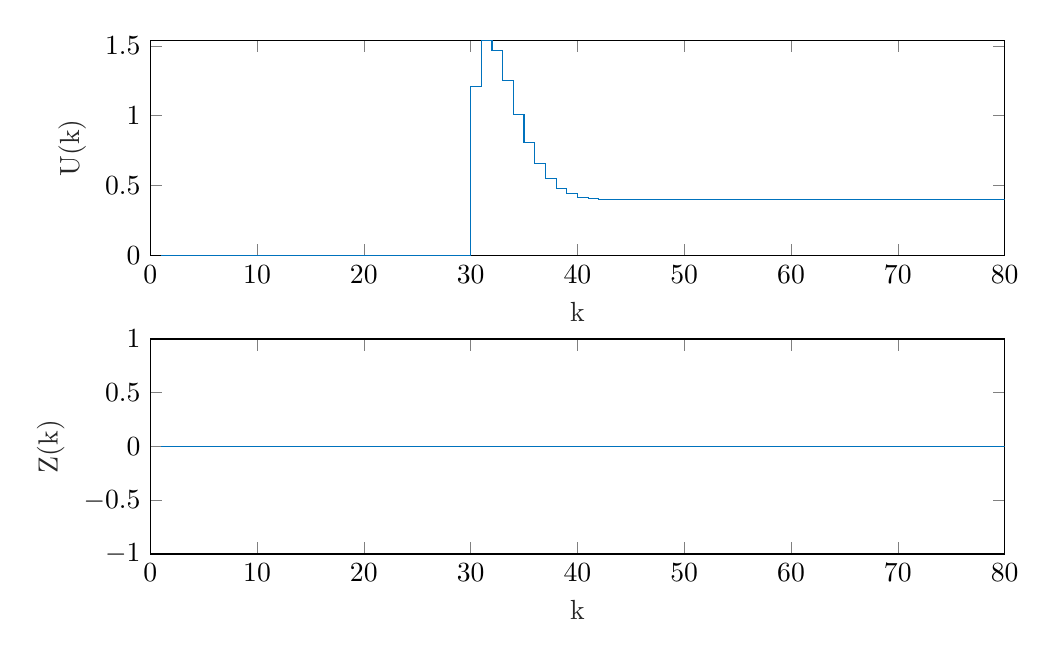
\begin{tikzpicture}

\begin{axis}[%
width=4.272in,
height=1.075in,
at={(0.717in,1.839in)},
scale only axis,
xmin=0,
xmax=80,
xlabel style={font=\color{white!15!black}},
xlabel={k},
ymin=0,
ymax=1.538576433506,
ylabel style={font=\color{white!15!black}},
ylabel={U(k)},
axis background/.style={fill=white}
]
\addplot[const plot, color=mycolor1, forget plot] table[row sep=crcr] {%
1	0\\
2	0\\
3	0\\
4	0\\
5	0\\
6	0\\
7	0\\
8	0\\
9	0\\
10	0\\
11	0\\
12	0\\
13	0\\
14	0\\
15	0\\
16	0\\
17	0\\
18	0\\
19	0\\
20	0\\
21	0\\
22	0\\
23	0\\
24	0\\
25	0\\
26	0\\
27	0\\
28	0\\
29	0\\
30	1.20577393725138\\
31	1.538576433506\\
32	1.46712127199355\\
33	1.24868968296282\\
34	1.01114447937986\\
35	0.808413088923491\\
36	0.655593901391529\\
37	0.54975127059157\\
38	0.481347710796871\\
39	0.4399381217831\\
40	0.416581469792359\\
41	0.404525444762055\\
42	0.399086664830369\\
43	0.397234397851693\\
44	0.397131373389285\\
45	0.397739526004153\\
46	0.39852169972768\\
47	0.39923446155087\\
48	0.39979385972787\\
49	0.400193942132608\\
50	0.400460651022531\\
51	0.400627917253023\\
52	0.40072678887092\\
53	0.400781648510957\\
54	0.400809906317153\\
55	0.40082312096247\\
56	0.400828485130777\\
57	0.40083019020383\\
58	0.400830499953435\\
59	0.400830517872924\\
60	0.400830696699621\\
61	0.400831155277304\\
62	0.400831862848653\\
63	0.400832738153988\\
64	0.400833697241719\\
65	0.400834672527807\\
66	0.400835617131571\\
67	0.400836502651825\\
68	0.400837314775299\\
69	0.400838048836104\\
70	0.400838706169384\\
71	0.400839291448234\\
72	0.400839810901075\\
73	0.40084027120997\\
74	0.400840678887897\\
75	0.400841039968263\\
76	0.400841359883766\\
77	0.400841643451092\\
78	0.400841894908521\\
79	0.400842117975164\\
80	0.400842315914761\\
};
\end{axis}

\begin{axis}[%
width=4.272in,
height=1.075in,
at={(0.717in,0.346in)},
scale only axis,
xmin=0,
xmax=80,
xlabel style={font=\color{white!15!black}},
xlabel={k},
ymin=-1,
ymax=1,
ylabel style={font=\color{white!15!black}},
ylabel={Z(k)},
axis background/.style={fill=white}
]
\addplot[const plot, color=mycolor1, forget plot] table[row sep=crcr] {%
1	0\\
2	0\\
3	0\\
4	0\\
5	0\\
6	0\\
7	0\\
8	0\\
9	0\\
10	0\\
11	0\\
12	0\\
13	0\\
14	0\\
15	0\\
16	0\\
17	0\\
18	0\\
19	0\\
20	0\\
21	0\\
22	0\\
23	0\\
24	0\\
25	0\\
26	0\\
27	0\\
28	0\\
29	0\\
30	0\\
31	0\\
32	0\\
33	0\\
34	0\\
35	0\\
36	0\\
37	0\\
38	0\\
39	0\\
40	0\\
41	0\\
42	0\\
43	0\\
44	0\\
45	0\\
46	0\\
47	0\\
48	0\\
49	0\\
50	0\\
51	0\\
52	0\\
53	0\\
54	0\\
55	0\\
56	0\\
57	0\\
58	0\\
59	0\\
60	0\\
61	0\\
62	0\\
63	0\\
64	0\\
65	0\\
66	0\\
67	0\\
68	0\\
69	0\\
70	0\\
71	0\\
72	0\\
73	0\\
74	0\\
75	0\\
76	0\\
77	0\\
78	0\\
79	0\\
80	0\\
};
\end{axis}
\end{tikzpicture}%
\caption{Zakłócenie i sygnał sterujący przy parametrach regulatora: $N=50$ $N_u=2$ $\lambda=0,4$}
\end{figure}

\begin{figure}[H]
\centering
\input{rysunki/strojenie_50_2_4.000000e-01_8.312159e+00.tex}
\caption{Wyjście obiektu przy parametrach regulatora: $N=50$ $N_u=2$ $\lambda=0,4$, błąd $E=8,312159$}
\end{figure}

\section{Wnioski}
Jak można było powyżej zauważyć, regulator DMC od samego początku działał w sposób dobry (błąd wynosił E=8,809637).
Zmiany parametru N nie dawały przez dłuższy czas zauważalnych zmian w przebiegach jak i w błędzie (dopiero przy N=20 błąd delikatnie wzrósł).
Przy modyfikacji parametru $N_U$ można było zaobserwować większą poprawę regulacji. Dla $N_U=5$ wskaźnik jakości regulacji oraz uchyb zmalały.
Jednak aby całkiem wyeliminiować uchyb zmniejszono $N_U$ do wartości 2, co spowodowało spowolnienie regulacji i tym samym wzrost błędu. 
Zmniejszenie warości współczynika lambda do wartości 0,4 przyśpieszyło regulację.

Najbardziej satysfakcjonujące wyniki uzyskano dla: $N_U=50$ $N=2$ $\lambda=0,4$. Dla tak dobranych parametrów wskaźnik jakości regulacji wynosił E=8,312159.

\smallskip

